\documentclass{article}
\usepackage[T1]{fontenc}
\usepackage{lmodern}
\usepackage{graphicx}
\usepackage{amsmath,amssymb}
\usepackage[a4paper,margin=2cm]{geometry}
\usepackage[absolute,overlay]{textpos}
\setlength{\TPHorizModule}{1mm}
\setlength{\TPVertModule}{1mm}
\usepackage[indonesian]{babel}
\usepackage{hyperref}
\setlength{\emergencystretch}{2em}
% unit: Halaman 84

\begin{document}

% === Halaman 84 (llm) ===

\vspace{279.18mm}

\vspace{10mm}
\begin{itemize}
    \item Dengan menggunakan tabel frekuensi kemunculan pasangan huruf di dalam Bahasa Inggris dan cipherteks yang cukup banyak, \textit{Playfair cipher} dapat dipecahkan.
    \item Kelemahan lainnya, bigram dan kebalikannya (misal AB dan BA) akan didekripsi menjadi pola huruf plainteks yang sama (misal RE dan ER). Di dalam bahasa Inggris terdapat banyak kata yang mengandung bigram terbalik seperti REceivER dan DEpartED.
\end{itemize}

% deskripsi: Grafik batang distribusi bigram yang menunjukkan frekuensi kemunculan pasangan huruf dalam bahasa Inggris, dengan 'TH' sebagai yang paling sering muncul.
% bbox normalisasi: [0.0000, 0.0000, 0.3200, 0.9400]
\begin{textblock*}{67.20mm}(0.00mm,0.00mm)
\noindent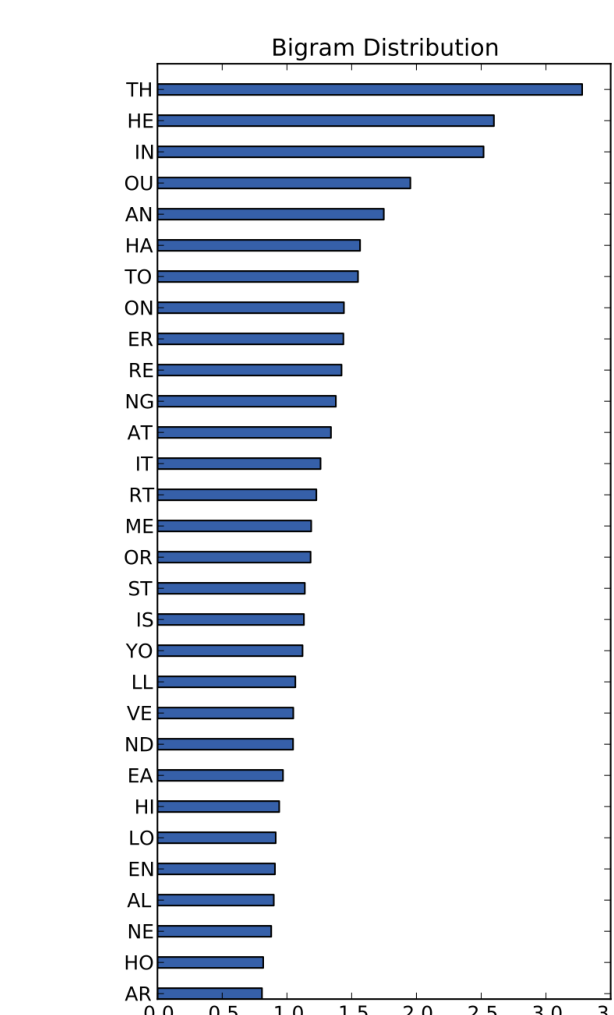
\includegraphics[width=67.20mm,height=279.18mm]{../../images/llm/page_084_img_01.png}%
\end{textblock*}

\end{document}
